%%________________________________________________________________________
%% LEIM | PROJETO
%% 2026 / 2022 / 2013 / 2012
%% Modelo para relatório
%% v05: alteração DEETC para DEI; outros ajustes
%% v04: alteração ADEETC para DEETC; outros ajustes
%% v03: correção de gralhas
%% v02: inclui anexo sobre utilização sistema controlo de versões
%% v01: original
%% PTS / MAR.2022 / MAI.2013 / 23.MAI.2012 (construído)
%%________________________________________________________________________




%%________________________________________________________________________
\chapter{Diagrama de Navegação da Interface}
\label{ch:outroDetalheAdicional}
%%________________________________________________________________________

\begin{figure}[h]
   \centering
   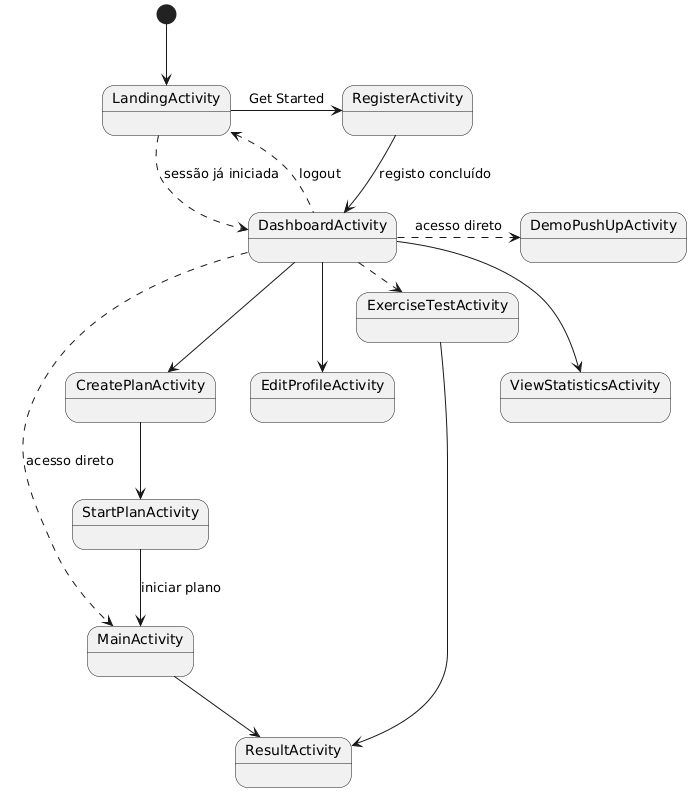
\includegraphics[width=\linewidth]{figuras/Diagrama_navegação.png}
   \caption{Fluxo de navegação entre os principais ecrãs da aplicação, referido na Secção \ref{sec:modulosCodigo}. Por clareza, omite-se o \texttt{LoaderActivity} (ecrã de transição genérico com \textit{spinner}), usado tanto pelo \texttt{LandingActivity} quando já existe sessão iniciada como pelo \texttt{DashboardActivity} no acesso direto a treinos (\texttt{MainActivity}, \texttt{DemoPushUpActivity}, \texttt{ExerciseTestActivity}). O \texttt{DemoPushUpActivity} é uma demo de duração fixa e atualmente não tem ecrã de resultado.}
   \label{fig:umlNavegacao}
\end{figure}








